% Options for packages loaded elsewhere
\PassOptionsToPackage{unicode}{hyperref}
\PassOptionsToPackage{hyphens}{url}
%
\documentclass[
]{book}
\usepackage{lmodern}
\usepackage{amssymb,amsmath}
\usepackage{ifxetex,ifluatex}
\ifnum 0\ifxetex 1\fi\ifluatex 1\fi=0 % if pdftex
  \usepackage[T1]{fontenc}
  \usepackage[utf8]{inputenc}
  \usepackage{textcomp} % provide euro and other symbols
\else % if luatex or xetex
  \usepackage{unicode-math}
  \defaultfontfeatures{Scale=MatchLowercase}
  \defaultfontfeatures[\rmfamily]{Ligatures=TeX,Scale=1}
\fi
% Use upquote if available, for straight quotes in verbatim environments
\IfFileExists{upquote.sty}{\usepackage{upquote}}{}
\IfFileExists{microtype.sty}{% use microtype if available
  \usepackage[]{microtype}
  \UseMicrotypeSet[protrusion]{basicmath} % disable protrusion for tt fonts
}{}
\makeatletter
\@ifundefined{KOMAClassName}{% if non-KOMA class
  \IfFileExists{parskip.sty}{%
    \usepackage{parskip}
  }{% else
    \setlength{\parindent}{0pt}
    \setlength{\parskip}{6pt plus 2pt minus 1pt}}
}{% if KOMA class
  \KOMAoptions{parskip=half}}
\makeatother
\usepackage{xcolor}
\IfFileExists{xurl.sty}{\usepackage{xurl}}{} % add URL line breaks if available
\IfFileExists{bookmark.sty}{\usepackage{bookmark}}{\usepackage{hyperref}}
\hypersetup{
  pdftitle={EDV1},
  pdfauthor={Max Brede},
  hidelinks,
  pdfcreator={LaTeX via pandoc}}
\urlstyle{same} % disable monospaced font for URLs
\usepackage{color}
\usepackage{fancyvrb}
\newcommand{\VerbBar}{|}
\newcommand{\VERB}{\Verb[commandchars=\\\{\}]}
\DefineVerbatimEnvironment{Highlighting}{Verbatim}{commandchars=\\\{\}}
% Add ',fontsize=\small' for more characters per line
\usepackage{framed}
\definecolor{shadecolor}{RGB}{248,248,248}
\newenvironment{Shaded}{\begin{snugshade}}{\end{snugshade}}
\newcommand{\AlertTok}[1]{\textcolor[rgb]{0.94,0.16,0.16}{#1}}
\newcommand{\AnnotationTok}[1]{\textcolor[rgb]{0.56,0.35,0.01}{\textbf{\textit{#1}}}}
\newcommand{\AttributeTok}[1]{\textcolor[rgb]{0.77,0.63,0.00}{#1}}
\newcommand{\BaseNTok}[1]{\textcolor[rgb]{0.00,0.00,0.81}{#1}}
\newcommand{\BuiltInTok}[1]{#1}
\newcommand{\CharTok}[1]{\textcolor[rgb]{0.31,0.60,0.02}{#1}}
\newcommand{\CommentTok}[1]{\textcolor[rgb]{0.56,0.35,0.01}{\textit{#1}}}
\newcommand{\CommentVarTok}[1]{\textcolor[rgb]{0.56,0.35,0.01}{\textbf{\textit{#1}}}}
\newcommand{\ConstantTok}[1]{\textcolor[rgb]{0.00,0.00,0.00}{#1}}
\newcommand{\ControlFlowTok}[1]{\textcolor[rgb]{0.13,0.29,0.53}{\textbf{#1}}}
\newcommand{\DataTypeTok}[1]{\textcolor[rgb]{0.13,0.29,0.53}{#1}}
\newcommand{\DecValTok}[1]{\textcolor[rgb]{0.00,0.00,0.81}{#1}}
\newcommand{\DocumentationTok}[1]{\textcolor[rgb]{0.56,0.35,0.01}{\textbf{\textit{#1}}}}
\newcommand{\ErrorTok}[1]{\textcolor[rgb]{0.64,0.00,0.00}{\textbf{#1}}}
\newcommand{\ExtensionTok}[1]{#1}
\newcommand{\FloatTok}[1]{\textcolor[rgb]{0.00,0.00,0.81}{#1}}
\newcommand{\FunctionTok}[1]{\textcolor[rgb]{0.00,0.00,0.00}{#1}}
\newcommand{\ImportTok}[1]{#1}
\newcommand{\InformationTok}[1]{\textcolor[rgb]{0.56,0.35,0.01}{\textbf{\textit{#1}}}}
\newcommand{\KeywordTok}[1]{\textcolor[rgb]{0.13,0.29,0.53}{\textbf{#1}}}
\newcommand{\NormalTok}[1]{#1}
\newcommand{\OperatorTok}[1]{\textcolor[rgb]{0.81,0.36,0.00}{\textbf{#1}}}
\newcommand{\OtherTok}[1]{\textcolor[rgb]{0.56,0.35,0.01}{#1}}
\newcommand{\PreprocessorTok}[1]{\textcolor[rgb]{0.56,0.35,0.01}{\textit{#1}}}
\newcommand{\RegionMarkerTok}[1]{#1}
\newcommand{\SpecialCharTok}[1]{\textcolor[rgb]{0.00,0.00,0.00}{#1}}
\newcommand{\SpecialStringTok}[1]{\textcolor[rgb]{0.31,0.60,0.02}{#1}}
\newcommand{\StringTok}[1]{\textcolor[rgb]{0.31,0.60,0.02}{#1}}
\newcommand{\VariableTok}[1]{\textcolor[rgb]{0.00,0.00,0.00}{#1}}
\newcommand{\VerbatimStringTok}[1]{\textcolor[rgb]{0.31,0.60,0.02}{#1}}
\newcommand{\WarningTok}[1]{\textcolor[rgb]{0.56,0.35,0.01}{\textbf{\textit{#1}}}}
\usepackage{longtable,booktabs}
% Correct order of tables after \paragraph or \subparagraph
\usepackage{etoolbox}
\makeatletter
\patchcmd\longtable{\par}{\if@noskipsec\mbox{}\fi\par}{}{}
\makeatother
% Allow footnotes in longtable head/foot
\IfFileExists{footnotehyper.sty}{\usepackage{footnotehyper}}{\usepackage{footnote}}
\makesavenoteenv{longtable}
\usepackage{graphicx}
\makeatletter
\def\maxwidth{\ifdim\Gin@nat@width>\linewidth\linewidth\else\Gin@nat@width\fi}
\def\maxheight{\ifdim\Gin@nat@height>\textheight\textheight\else\Gin@nat@height\fi}
\makeatother
% Scale images if necessary, so that they will not overflow the page
% margins by default, and it is still possible to overwrite the defaults
% using explicit options in \includegraphics[width, height, ...]{}
\setkeys{Gin}{width=\maxwidth,height=\maxheight,keepaspectratio}
% Set default figure placement to htbp
\makeatletter
\def\fps@figure{htbp}
\makeatother
\setlength{\emergencystretch}{3em} % prevent overfull lines
\providecommand{\tightlist}{%
  \setlength{\itemsep}{0pt}\setlength{\parskip}{0pt}}
\setcounter{secnumdepth}{5}
\usepackage{booktabs}
\usepackage{booktabs}
\usepackage{longtable}
\usepackage{array}
\usepackage{multirow}
\usepackage{wrapfig}
\usepackage{float}
\usepackage{colortbl}
\usepackage{pdflscape}
\usepackage{tabu}
\usepackage{threeparttable}
\usepackage{threeparttablex}
\usepackage[normalem]{ulem}
\usepackage{makecell}
\usepackage{xcolor}
\ifluatex
  \usepackage{selnolig}  % disable illegal ligatures
\fi
\usepackage[]{natbib}
\bibliographystyle{apalike}

\title{EDV1}
\author{Max Brede}
\date{2020-10-30}

\begin{document}
\maketitle

{
\setcounter{tocdepth}{1}
\tableofcontents
}
\hypertarget{vorwort}{%
\chapter{Vorwort}\label{vorwort}}

Dieses mit \texttt{bookdown} erstellte Dokument ist das über das Wintersemester 2020 hinweg wachsende Skript zur Übung ``PSY\_B\_11-2: Computerunterstützte Datenanalyse I'' der CAU zu Kiel.

\hypertarget{lehrplan}{%
\chapter{Lehrplan}\label{lehrplan}}

\hypertarget{semesterplan}{%
\section{Semesterplan}\label{semesterplan}}

\hypertarget{uxfcbungsformat}{%
\section{Übungsformat}\label{uxfcbungsformat}}

Die Übung soll zur Hälfte in 45-minütigen Sitzungen im Vorlesungsformat zur Vorstellung der Funktionen und zur anderen Hälfte als 45-minütige praktische Übung stattfinden.
Es wird pro Übungs-Sitzung ein Übungszettel ausgegeben, der mit Hilfe der in der Zugehörigen Vorlesung besprochenen Funktionen bearbeitet werden können soll.
Diese Zettel sollen nach der jeweiligen Vorlesung für die Übungen vorbereitet werden, in denen der Zettel dann besprochen und mögliche Fragen geklärt werden.
Nach den Übungssitzungen haben die Studierenden dann eine Woche Zeit, zusätzliche Hausaufgaben zu bearbeiten.

Eine Ausnahme von diesem Ablauf ist die erste Sitzung, in der organisatorisches und Grundlagen in 90 minütigem Vorlesungsstil besprochen werden sollen. Auch nach dieser Sitzung werden aber Übungszettel und Hausaufgaben ausgegeben.

\hypertarget{lehrziele-fuxfcr-jede-sitzung}{%
\section{Lehrziele für jede Sitzung}\label{lehrziele-fuxfcr-jede-sitzung}}

Die Studierenden können nach dem Absolvieren der Übung\ldots{}

\hypertarget{einheit-1}{%
\subsubsection*{Einheit 1}\label{einheit-1}}
\addcontentsline{toc}{subsubsection}{Einheit 1}

\begin{itemize}
\tightlist
\item
  Vor- und Nachteile von R und RStudio nennen und diese installieren.
\item
  erklären was Funktionen und was Argumente sind.
\item
  die Hilfe benutzen.
\item
  das Environment von R benutzen um Objekte anzulegen und zu löschen.
\end{itemize}

\hypertarget{einheit-2}{%
\subsubsection*{Einheit 2}\label{einheit-2}}
\addcontentsline{toc}{subsubsection}{Einheit 2}

\begin{itemize}
\tightlist
\item
  Vektoren erstellen, tranformieren und indizieren.
\item
  verschiedene Datenformate in R erstellen, benutzen und in einander überführen.
\end{itemize}

\hypertarget{einheit-3}{%
\subsubsection*{Einheit 3}\label{einheit-3}}
\addcontentsline{toc}{subsubsection}{Einheit 3}

\begin{itemize}
\tightlist
\item
  Pakete installieren und benutzen.
\item
  mit Hilfe des ``\texttt{tidyverse}'' Datensätze erstellen, ergänzen, sortieren und indizieren.
\end{itemize}

\hypertarget{einheit-4}{%
\subsubsection*{Einheit 4}\label{einheit-4}}
\addcontentsline{toc}{subsubsection}{Einheit 4}

\begin{itemize}
\tightlist
\item
  Faktoren erstellen.
\item
  deskriptive Kennwerte berechnen.
\item
  Daten auf Gruppenebene aggregieren.
\end{itemize}

\hypertarget{einheit-5}{%
\subsubsection*{Einheit 5}\label{einheit-5}}
\addcontentsline{toc}{subsubsection}{Einheit 5}

\begin{itemize}
\tightlist
\item
  Daten auf Gruppenebene noch besser aggregieren.
\item
  Häufigkeiten auszählen und tabellarisch darstellen.
\item
  Datensätze aus verschiedenen Formaten einlesen.
\end{itemize}

\hypertarget{einheit-6}{%
\subsubsection*{Einheit 6}\label{einheit-6}}
\addcontentsline{toc}{subsubsection}{Einheit 6}

\begin{itemize}
\tightlist
\item
  eine Anzahl von Grafiken erstellen.
\end{itemize}

\hypertarget{einheit-7}{%
\subsubsection*{Einheit 7}\label{einheit-7}}
\addcontentsline{toc}{subsubsection}{Einheit 7}

\begin{itemize}
\tightlist
\item
  kompliziertere Grafiken erstellen.
\end{itemize}

\hypertarget{einheit-8}{%
\subsubsection*{Einheit 8}\label{einheit-8}}
\addcontentsline{toc}{subsubsection}{Einheit 8}

\begin{itemize}
\tightlist
\item
  die Funktionsschreibweise lesen und anwenden.
\item
  erfolfreich an der Klausur teilnehmen.
\end{itemize}

\hypertarget{pruxfcfungsleistung}{%
\section{Prüfungsleistung}\label{pruxfcfungsleistung}}

Die Studierenden \textbf{müssen} während des Semesters die nach den Übungssitzungen ausgegebenen Hausaufgaben innerhalb einer Woche sinnvoll bearbeitet abgeben.

Mit maximal einer nicht sinnvoll bearbeiteten Serie werden die Studierenden zur Klausur am Ende des Semesters zugelassen.

\hypertarget{vorlesung-i---rste-schritte}{%
\chapter{Vorlesung I - Rste Schritte}\label{vorlesung-i---rste-schritte}}

\hypertarget{organisatorisches}{%
\section{Organisatorisches}\label{organisatorisches}}

\hypertarget{semesterplan-1}{%
\subsection*{Semesterplan}\label{semesterplan-1}}
\addcontentsline{toc}{subsection}{Semesterplan}

\begin{table}[H]
\centering\begingroup\fontsize{15}{17}\selectfont

\begin{tabular}{l|l|l|l}
\hline
Einheit & Vorlesung & Übungswoche & Thema\\
\hline
1 & 2.11.20 & keine Übung & Grundlagen und Begriffe\\
\hline
2 & 16.11.20 & KW 48 & Vektoren und Indizierung\\
\hline
 &  &  & Datenformate erstellen und transformieren\\
\hline
3 & 30.11.20 & KW 50 & Pakete installieren und benutzen\\
\hline
 &  &  & Datensätze erstellen und ergänzen können\\
\hline
 &  &  & Datensätze sortieren und indizieren können\\
\hline
4 & 14.12.20 & KW 1 & Faktoren\\
\hline
 &  &  & deskriptive Kennwerte\\
\hline
 &  &  & Aggregation I\\
\hline
5 & 11.01.21 & KW 3 & Aggregation II\\
\hline
 &  &  & In- und Export von Datensätzen\\
\hline
6 & 25.01.21 & KW 5 & Grafische Darstellungen I\\
\hline
7 & 08.02.21 & KW 7 & Grafische Darstellungen II\\
\hline
8 & 22.02.21 & keine Übung & Puffer\\
\hline
 &  &  & Probeklausur\\
\hline
\end{tabular}
\endgroup{}
\end{table}

\hypertarget{uxfcbungsablauf}{%
\subsection*{Übungsablauf}\label{uxfcbungsablauf}}
\addcontentsline{toc}{subsection}{Übungsablauf}

Die Übung wird zur Hälfte als Vorlesung, zur anderen Hälfte in Kleingruppen abgehalten.

Die Daten sind im Kalender und im Semesterplan im Olat ersichtlich.

\hypertarget{pruxfcfungsleistung-1}{%
\subsection*{Prüfungsleistung}\label{pruxfcfungsleistung-1}}
\addcontentsline{toc}{subsection}{Prüfungsleistung}

Die Prüfungsleistung in dieser Veranstaltung besteht aus:

\begin{enumerate}
\def\labelenumi{\arabic{enumi}.}
\tightlist
\item
  Dem \emph{regelmäßigen Bearbeiten} und \emph{Bestehen} von Hausaufgaben. Diese werden über das OLAT ausgeteilt und abgegeben, zu jeder Veranstaltung wird eine neue Serie herausgegeben. Das Bestehen der Hausaufgaben ist nötig, um zur Klausur zugelassen zu werden.

  \begin{itemize}
  \tightlist
  \item
    Als \emph{Bestanden} gilt eine Serie, wenn alle Aufgaben \textbf{sinnvoll} bearbeitet wurden.
  \item
    Unter \emph{regelmäßigem Bearbeiten} versteht sich das Bestehen aller Serien \textbf{mit einer Ausnahme}. \medskip  
  \end{itemize}
\item
  Im Klausurzeitraum findet an einem Tag eine praktische Prüfung statt.
\end{enumerate}

\hypertarget{einfuxfchrung}{%
\section{Einführung}\label{einfuxfchrung}}

\hypertarget{rste-schritte}{%
\subsection*{Rste Schritte}\label{rste-schritte}}
\addcontentsline{toc}{subsection}{Rste Schritte}

Diese Veranstaltung und das zugehörige Material sollen Ihnen einen Einstieg in das computergestützte Aufbereiten und Auswerten von empirischen Daten bieten.
Dazu werden wir auf die von ihren Autoren als `software environment for statistical computing and graphics' bezeichnete, freie Umgebung R zurückgreifen.

\hypertarget{wozu-brauche-ich-das}{%
\subsection*{Wozu brauche ich das?}\label{wozu-brauche-ich-das}}
\addcontentsline{toc}{subsection}{Wozu brauche ich das?}

\begin{center}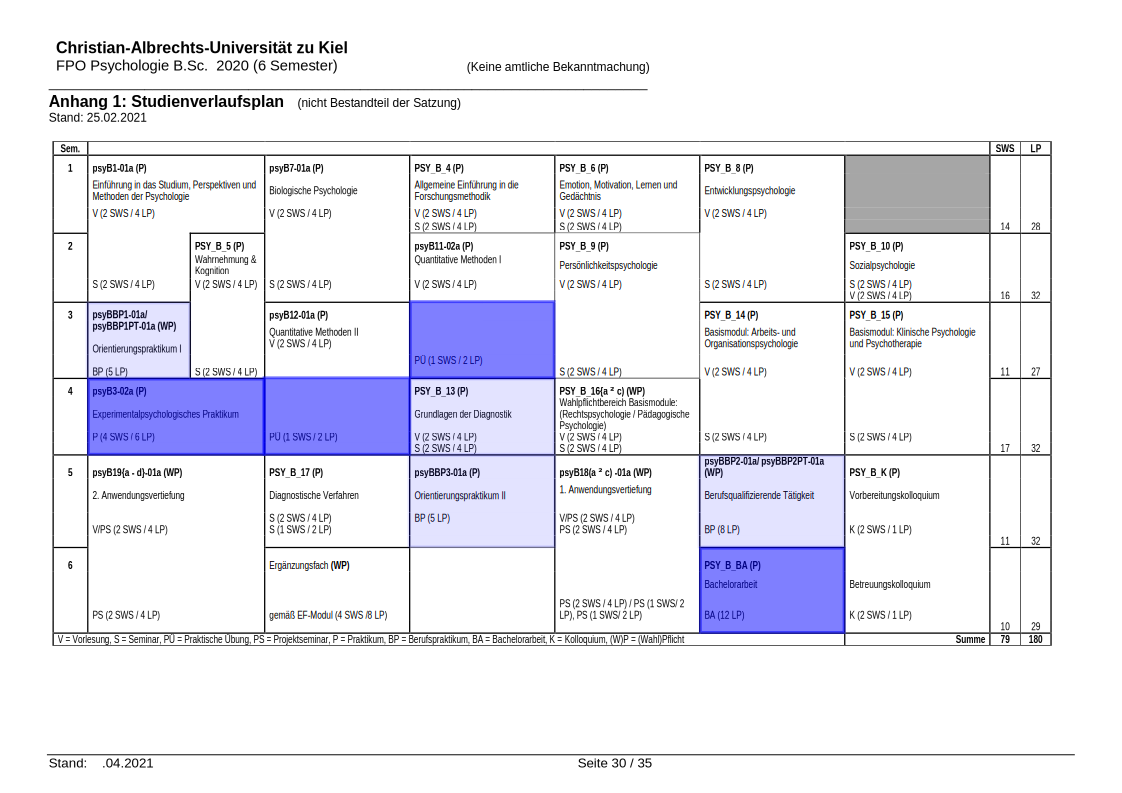
\includegraphics[width=0.8\linewidth]{imgs/relevanz} \end{center}

\hypertarget{warum-r}{%
\subsection*{Warum R ?}\label{warum-r}}
\addcontentsline{toc}{subsection}{Warum R ?}

\hypertarget{und-nicht-spss}{%
\subsubsection*{(\ldots und nicht SPSS\ldots)}\label{und-nicht-spss}}
\addcontentsline{toc}{subsubsection}{(\ldots und nicht SPSS\ldots)}

\begin{table}[H]
\centering
\begin{tabular}[t]{l|l|l}
\hline
  & SPSS & R\\
\hline
 &  & \\
\hline
Pro & einfache Bedienung & das `CRAN` (Comprehensive R Archive Network)\\
\hline
 & weit verbreitet & kostenlos\\
\hline
 &  & macht was angewiesen ist\\
\hline
 &  & \\
\hline
Contra & kann nicht alles & etwas Gewöhnung notwendig\\
\hline
 & relativ kostenintensive Lizenzen & \\
\hline
 & nimmt vieles ab & \\
\hline
 & nicht beliebig erweiterbar & \\
\hline
\end{tabular}
\end{table}

Aber die viel wichtigeren Argumente:
R kann \textbf{Alles}

\begin{center}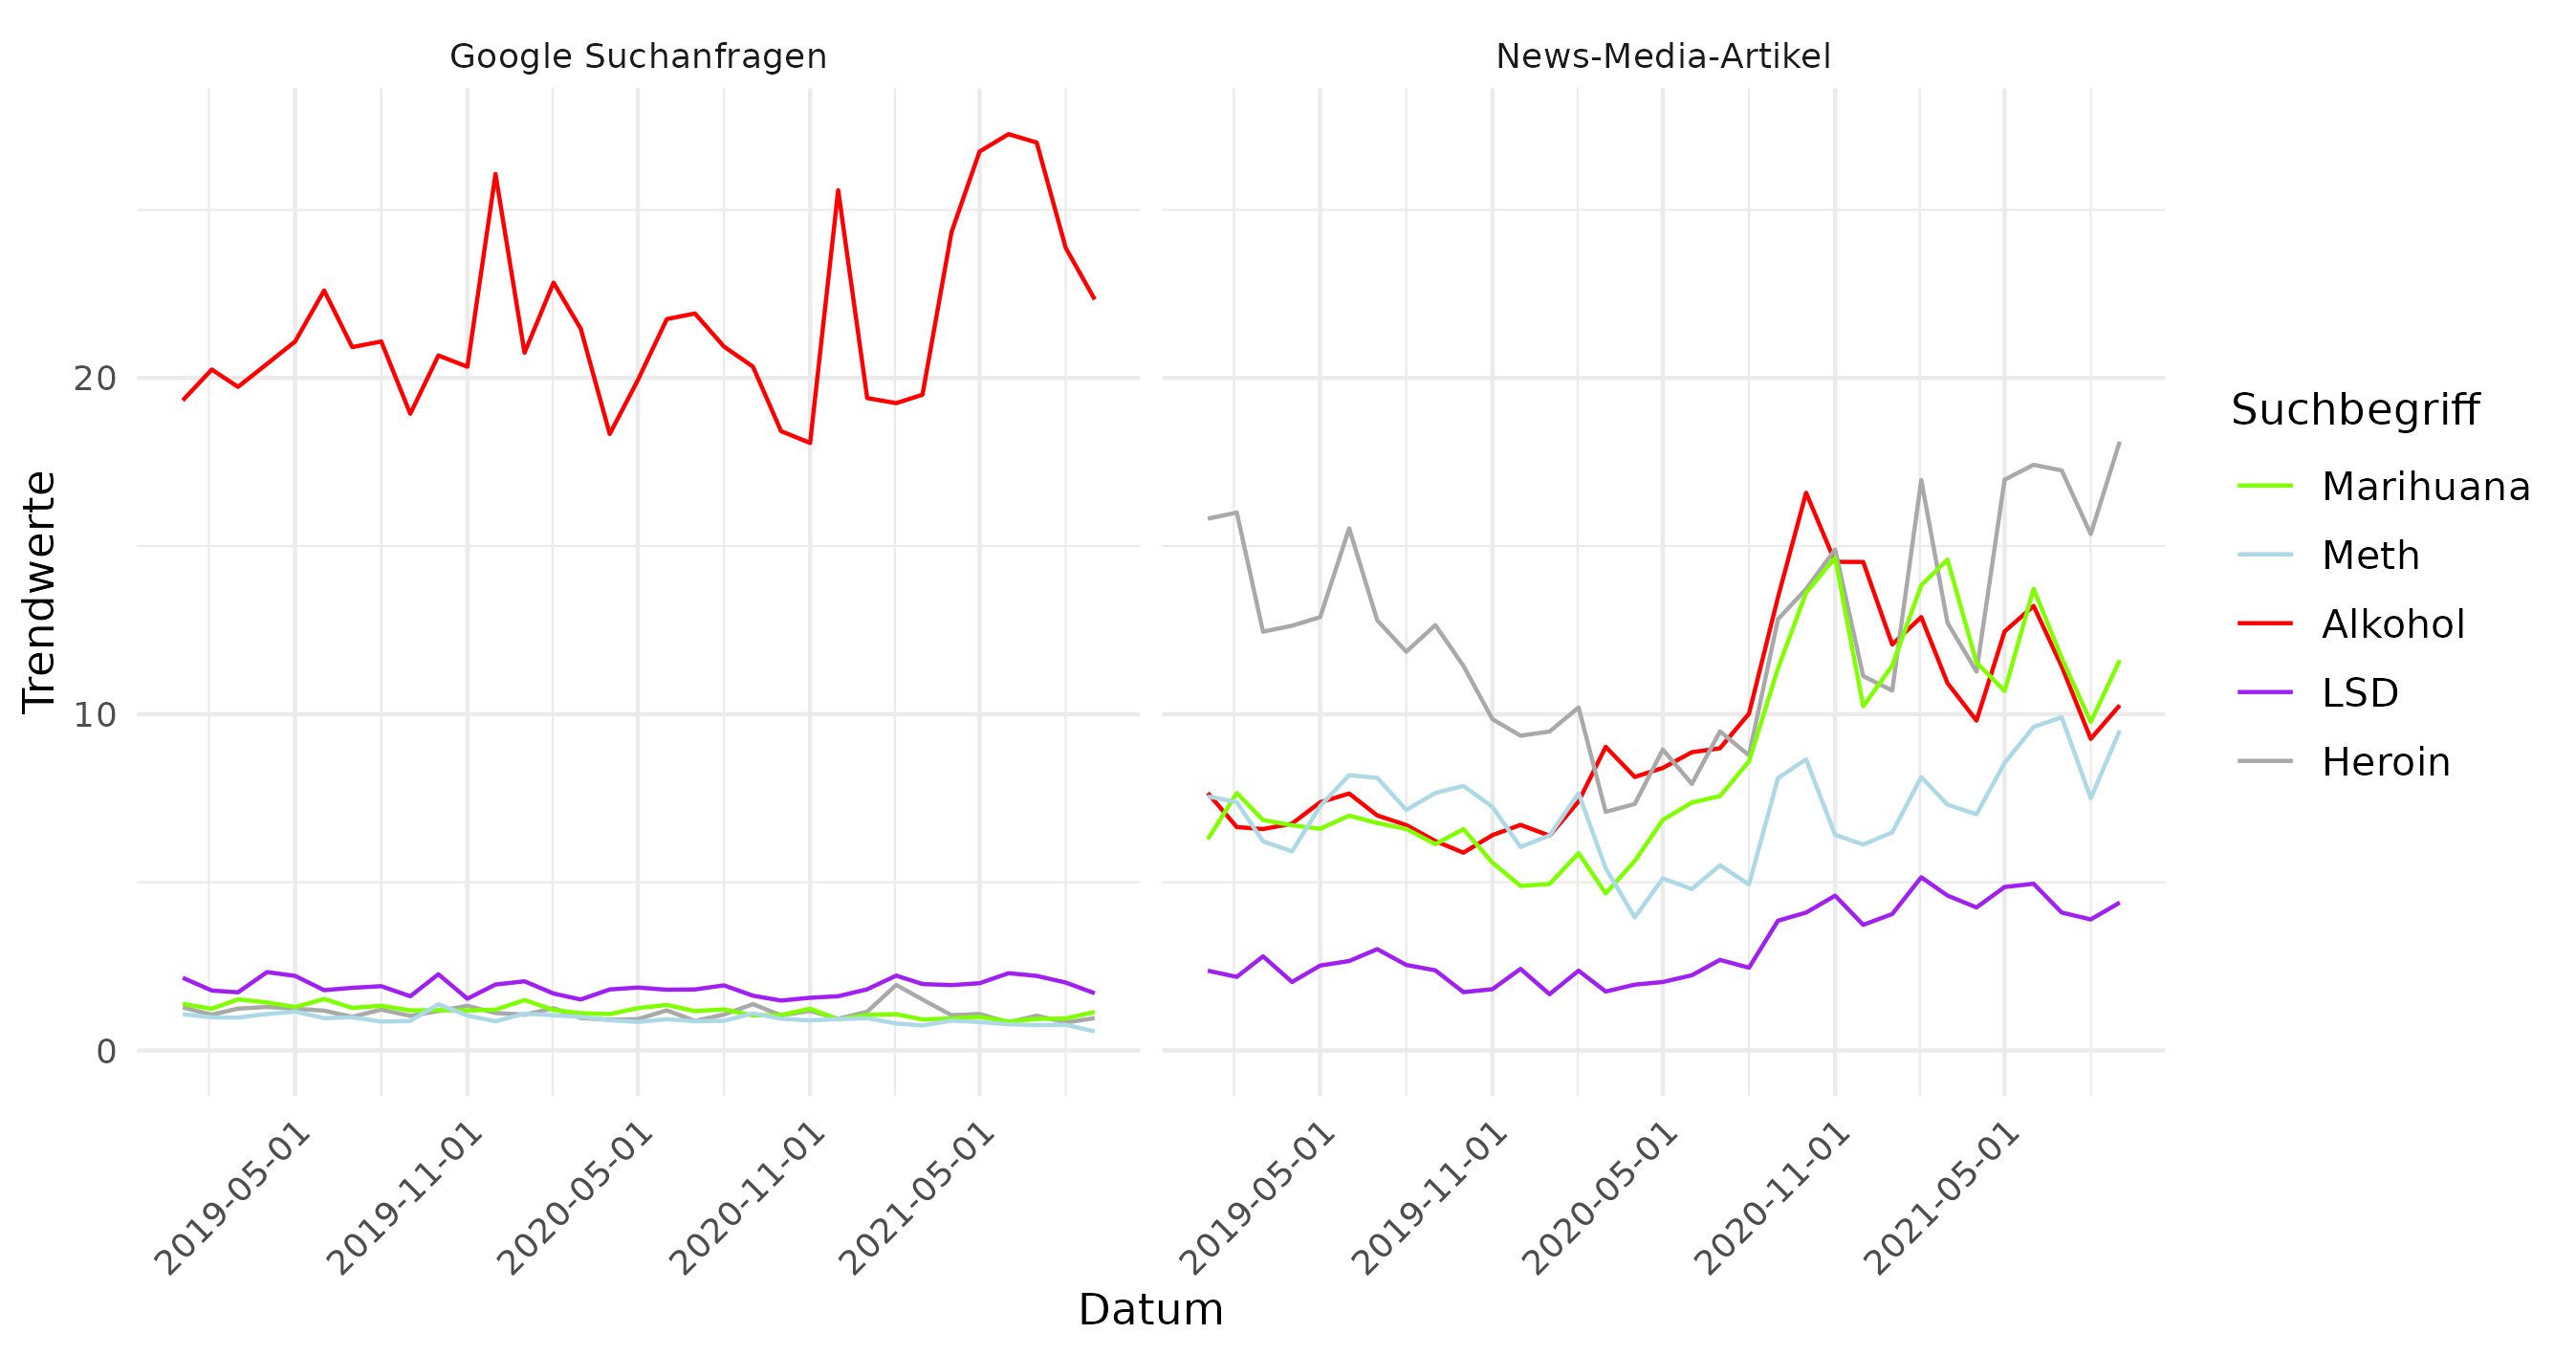
\includegraphics[width=0.7\linewidth]{imgs/drugs} \end{center}

R macht \textbf{Spass}

\begin{center}\includegraphics[width=0.45\linewidth]{imgs/thumbnail} \end{center}

\hypertarget{literatur}{%
\subsection*{Literatur}\label{literatur}}
\addcontentsline{toc}{subsection}{Literatur}

Die Veranstaltung orientiert sich an:

\begin{enumerate}
\def\labelenumi{\arabic{enumi}.}
\item
  \citet{wollschlaegerKompaktSchnelleEinstieg2016} . R kompakt.(Link aus dem Uni-Netz).
\item
  \citet{grolemundDataScience} . R for Data Science (Link).
\end{enumerate}

\hypertarget{installation-verwendung}{%
\subsection*{Installation \& Verwendung}\label{installation-verwendung}}
\addcontentsline{toc}{subsection}{Installation \& Verwendung}

Es wird die Verwendung der grafischen Benutzeroberfläche \href{http://www.rstudio.com}{RStudio} empfohlen.

Beachten Sie, dass für die Verwendung von RStudio zuvor eine Basisinstallation von \href{http://cran.r-project.org}{R} erfolgen muss:

\begin{enumerate}
\def\labelenumi{\arabic{enumi}.}
\item
  (R) herunterladen und installieren.
\item
  (RStudio) herunterladen und installieren.
\end{enumerate}

\hypertarget{benutzeroberfluxe4che-rstudio}{%
\subsection*{Benutzeroberfläche RStudio}\label{benutzeroberfluxe4che-rstudio}}
\addcontentsline{toc}{subsection}{Benutzeroberfläche RStudio}

\begin{figure}
\centering
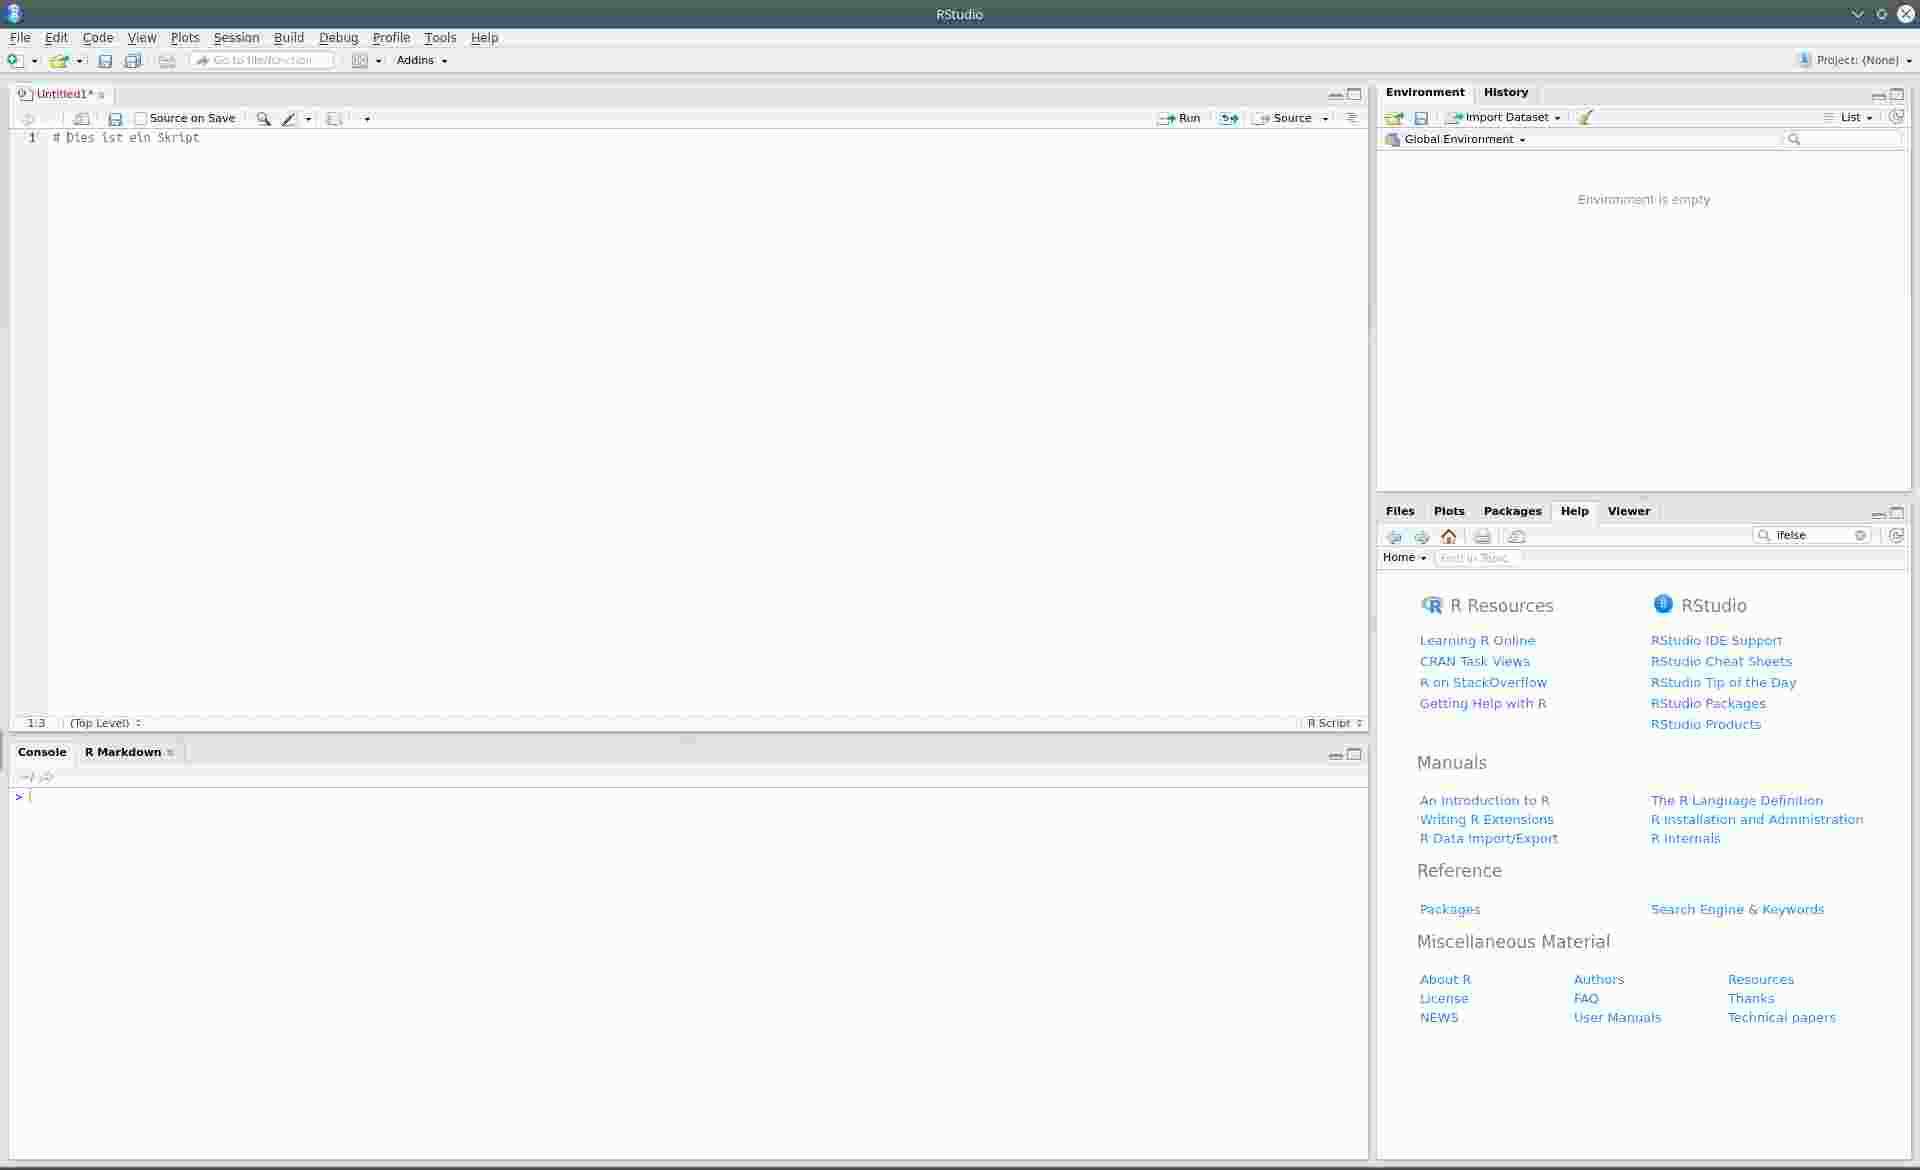
\includegraphics[width=0.6\textwidth,height=\textheight]{imgs/RStudio_003.jpg}
\caption{Benutzeroberfläche von RStudio. Oben links: Editor; unten links: Konsole; oben rechts: Environment bzw. History; unten rechts: Files, Plots, Help, etc.}
\end{figure}

\hypertarget{allgemeine-hinweise}{%
\subsection*{Allgemeine Hinweise}\label{allgemeine-hinweise}}
\addcontentsline{toc}{subsection}{Allgemeine Hinweise}

\begin{itemize}
\tightlist
\item
  Verwenden Sie die Konsole (unten links) nur für einzeilige Berechnungen beim ``Ausprobieren''
\item
  Verwenden Sie stets den Editor (oben links), um mehrzeilige Berechnungen direkt in ein Skript zu schreiben
\item
  Kommentieren Sie Ihren Code ausreichend und sinnvoll mit Hilfe des \texttt{\#}-Zeichens
\item
  Speichern Sie Ihr Skript unter einem sinnvollen Namen in einem sinnvoll benannten Verzeichnis ab
\end{itemize}

\begin{itemize}
\tightlist
\item
  Speichern Sie regelmäßig mit Strg+S zwischen
\item
  Eine einzelne Skript-Zeile (diejenige, in der sich der Cursor befindet) oder zuvor markierter Code lassen sich mit Strg+Enter ausführen
\item
  In der Konsole bricht ESC die Eingabe ab
\end{itemize}

\hypertarget{zum-besseren-verstuxe4ndnis}{%
\subsection*{Zum besseren Verständnis}\label{zum-besseren-verstuxe4ndnis}}
\addcontentsline{toc}{subsection}{Zum besseren Verständnis}

In diesem Skript enthalten die grau hinterlegten Zeilen R-Input, die weiß hinterlegten Zeilen den R-Output. Ein ganz einfaches Beispiel zum Ausprobieren: Die simple Berechnung von 1 + 1.

\begin{Shaded}
\begin{Highlighting}[]
\DecValTok{1} \OperatorTok{+}\StringTok{ }\DecValTok{1}
\end{Highlighting}
\end{Shaded}

\begin{verbatim}
## [1] 2
\end{verbatim}

\hypertarget{ausdruxfccke-in-der-r-konsole}{%
\subsection*{Ausdrücke in der R-Konsole}\label{ausdruxfccke-in-der-r-konsole}}
\addcontentsline{toc}{subsection}{Ausdrücke in der R-Konsole}

Anweisungen in R funktionieren grundsätzlich über das Ausführen von Ausdrücken. Dabei werden Ausdrücke entweder durch Semikolons oder Zeilenumbrüche beendet.

\begin{Shaded}
\begin{Highlighting}[]
\DecValTok{1} \OperatorTok{+}\StringTok{ }\DecValTok{1}\NormalTok{; }\DecValTok{2} \OperatorTok{+}\StringTok{ }\DecValTok{2}\NormalTok{;}
\end{Highlighting}
\end{Shaded}

\begin{verbatim}
## [1] 2
\end{verbatim}

\begin{verbatim}
## [1] 4
\end{verbatim}

\begin{Shaded}
\begin{Highlighting}[]
\DecValTok{1}\OperatorTok{+}\DecValTok{1}
\end{Highlighting}
\end{Shaded}

\begin{verbatim}
## [1] 2
\end{verbatim}

\begin{Shaded}
\begin{Highlighting}[]
\DecValTok{2}\OperatorTok{+}\DecValTok{2}
\end{Highlighting}
\end{Shaded}

\begin{verbatim}
## [1] 4
\end{verbatim}

\hypertarget{kommentare}{%
\subsection*{Kommentare}\label{kommentare}}
\addcontentsline{toc}{subsection}{Kommentare}

R bietet außerdem die Möglichkeit, im Code Anmerkungen zu machen, die beim Ausführen ignoriert werden. Diese werden mit einem \texttt{\#}-Symbol eingeleitet.

\begin{Shaded}
\begin{Highlighting}[]
\DecValTok{1} \OperatorTok{+}\StringTok{ }\DecValTok{1} \CommentTok{\#\#\# +1 +1}
\end{Highlighting}
\end{Shaded}

\begin{verbatim}
## [1] 2
\end{verbatim}

\begin{Shaded}
\begin{Highlighting}[]
\CommentTok{\#Dies ist ein Kommentar}
\end{Highlighting}
\end{Shaded}

Nutzen Sie Kommentare innerhalb Ihrer Skripte, um Arbeitsschritte kenntlich zu machen und zu erklären. Die übersichtliche Gestaltung Ihrer Skripte ist von wirklich großem Vorteil bei der Arbeit mit R. Dies kann nicht oft genug betont werden.

\hypertarget{grundlegende-rechenoperationen}{%
\section{Grundlegende Rechenoperationen}\label{grundlegende-rechenoperationen}}

\hypertarget{addition-subtraktion}{%
\subsection*{Addition, Subtraktion}\label{addition-subtraktion}}
\addcontentsline{toc}{subsection}{Addition, Subtraktion}

\begin{Shaded}
\begin{Highlighting}[]
\DecValTok{2} \OperatorTok{+}\StringTok{ }\DecValTok{3}  
\end{Highlighting}
\end{Shaded}

\begin{verbatim}
## [1] 5
\end{verbatim}

\begin{Shaded}
\begin{Highlighting}[]
\DecValTok{28} \OperatorTok{{-}}\StringTok{ }\DecValTok{5}  
\end{Highlighting}
\end{Shaded}

\begin{verbatim}
## [1] 23
\end{verbatim}

\hypertarget{multiplikation-division}{%
\subsection*{Multiplikation, Division}\label{multiplikation-division}}
\addcontentsline{toc}{subsection}{Multiplikation, Division}

\begin{Shaded}
\begin{Highlighting}[]
\DecValTok{2} \OperatorTok{*}\StringTok{ }\DecValTok{21}   
\end{Highlighting}
\end{Shaded}

\begin{verbatim}
## [1] 42
\end{verbatim}

\begin{Shaded}
\begin{Highlighting}[]
\DecValTok{92} \OperatorTok{/}\StringTok{ }\DecValTok{4}
\end{Highlighting}
\end{Shaded}

\begin{verbatim}
## [1] 23
\end{verbatim}

\hypertarget{rechenregeln}{%
\subsection*{Rechenregeln}\label{rechenregeln}}
\addcontentsline{toc}{subsection}{Rechenregeln}

\begin{Shaded}
\begin{Highlighting}[]
\DecValTok{1}\OperatorTok{+}\DecValTok{1}\OperatorTok{*}\DecValTok{1}\OperatorTok{+}\DecValTok{1}\OperatorTok{*}\NormalTok{(}\DecValTok{1}\OperatorTok{+}\DecValTok{1}\NormalTok{)}\OperatorTok{+}\DecValTok{1}
\end{Highlighting}
\end{Shaded}

\begin{verbatim}
## [1] 5
\end{verbatim}

Wie man sieht, befolgt R die Punkt-vor-Strich-Regel und berücksichtigt Klammerung.

\hypertarget{potenz-quadratwurzel-squareroot-betrag-absolute}{%
\subsection*{Potenz, Quadratwurzel (``squareroot''), Betrag (``absolute'')}\label{potenz-quadratwurzel-squareroot-betrag-absolute}}
\addcontentsline{toc}{subsection}{Potenz, Quadratwurzel (``squareroot''), Betrag (``absolute'')}

\begin{Shaded}
\begin{Highlighting}[]
\DecValTok{3}\OperatorTok{\^{}}\DecValTok{2}
\end{Highlighting}
\end{Shaded}

\begin{verbatim}
## [1] 9
\end{verbatim}

\begin{Shaded}
\begin{Highlighting}[]
\KeywordTok{sqrt}\NormalTok{(}\DecValTok{9}\NormalTok{)}
\end{Highlighting}
\end{Shaded}

\begin{verbatim}
## [1] 3
\end{verbatim}

\begin{Shaded}
\begin{Highlighting}[]
\KeywordTok{abs}\NormalTok{(}\OperatorTok{{-}}\DecValTok{42}\NormalTok{)}
\end{Highlighting}
\end{Shaded}

\begin{verbatim}
## [1] 42
\end{verbatim}

\hypertarget{runden}{%
\subsection*{Runden}\label{runden}}
\addcontentsline{toc}{subsection}{Runden}

\begin{Shaded}
\begin{Highlighting}[]
\NormalTok{pi}
\end{Highlighting}
\end{Shaded}

\begin{verbatim}
## [1] 3.141593
\end{verbatim}

\begin{Shaded}
\begin{Highlighting}[]
\KeywordTok{round}\NormalTok{(pi)}
\end{Highlighting}
\end{Shaded}

\begin{verbatim}
## [1] 3
\end{verbatim}

\begin{Shaded}
\begin{Highlighting}[]
\KeywordTok{round}\NormalTok{(pi, }\DataTypeTok{digits=}\DecValTok{2}\NormalTok{)}
\end{Highlighting}
\end{Shaded}

\begin{verbatim}
## [1] 3.14
\end{verbatim}

\begin{Shaded}
\begin{Highlighting}[]
\KeywordTok{round}\NormalTok{(pi, }\DataTypeTok{digits=}\DecValTok{3}\NormalTok{)}
\end{Highlighting}
\end{Shaded}

\begin{verbatim}
## [1] 3.142
\end{verbatim}

\hypertarget{aufgabe}{%
\subsection*{Aufgabe}\label{aufgabe}}
\addcontentsline{toc}{subsection}{Aufgabe}

\begin{Shaded}
\begin{Highlighting}[]
\KeywordTok{round}\NormalTok{(pi, }\DataTypeTok{digits =} \DecValTok{0}\NormalTok{) }\OperatorTok{*}\StringTok{ }\DecValTok{3} \CommentTok{\#\#\# + 5}
\end{Highlighting}
\end{Shaded}

\hypertarget{was-kommt-raus}{%
\subsubsection*{Was kommt raus?}\label{was-kommt-raus}}
\addcontentsline{toc}{subsubsection}{Was kommt raus?}

\begin{enumerate}
\def\labelenumi{\Alph{enumi})}
\tightlist
\item
  \texttt{pi}
\item
  \texttt{14}
\item
  eine Fehlermeldung
\item
  \texttt{9}
\item
  \texttt{NULL}
\end{enumerate}

\hypertarget{ausdruxfccke-funktionen-argumente}{%
\section{Ausdrücke, Funktionen, Argumente}\label{ausdruxfccke-funktionen-argumente}}

\hypertarget{funktionen-argumente}{%
\subsection*{Funktionen \& Argumente}\label{funktionen-argumente}}
\addcontentsline{toc}{subsection}{Funktionen \& Argumente}

In R werden sehr häufig \emph{Funktionen} verwendet. Diese repräsentieren eine Reihe von Anweisungen, die beim Aufrufen mit spezifischen Parametern ausgeführt werden sollen. Diese Parameter werde in Form von \emph{Argumenten} übergeben.
Beispielsweise enthält die Funktion \texttt{round()} die nötigen Anweisungen, um eine Zahl zu runden. Hierfür erwartet \texttt{round()} die zu rundende Zahl und die Anzahl an Nachkommastellen auf die zu runden ist.
Man schreibt immer \emph{Funktionsname}(\emph{Argumentliste}). Bei Funktionen müssen \emph{immer} runde Klammern vorhanden sein, auch wenn keine einzelnen Argumente vorgegeben werden.

Es gibt \emph{obligatorische Argumente}, ohne deren Übergabe das Aufrufen einer Funktion zu einer Fehlermeldung führt:
\scriptsize

\begin{Shaded}
\begin{Highlighting}[]
\KeywordTok{round}\NormalTok{(pi)}
\end{Highlighting}
\end{Shaded}

\begin{verbatim}
## [1] 3
\end{verbatim}

\begin{Shaded}
\begin{Highlighting}[]
\KeywordTok{round}\NormalTok{() }\CommentTok{\#\#\# Funktionsaufruf ohne Argument}
\end{Highlighting}
\end{Shaded}

\begin{verbatim}
## Error in eval(expr, envir, enclos): 0 arguments passed to 'round' which requires 1 or 2 arguments
\end{verbatim}

\ldots{} und \emph{optionale Argumente}:
\scriptsize

\begin{Shaded}
\begin{Highlighting}[]
\KeywordTok{round}\NormalTok{(pi, }\DataTypeTok{digits=}\DecValTok{3}\NormalTok{)}
\end{Highlighting}
\end{Shaded}

\begin{verbatim}
## [1] 3.142
\end{verbatim}

\begin{Shaded}
\begin{Highlighting}[]
\KeywordTok{round}\NormalTok{(pi, }\DataTypeTok{digits=}\NormalTok{pi)}
\end{Highlighting}
\end{Shaded}

\begin{verbatim}
## [1] 3.142
\end{verbatim}

\begin{Shaded}
\begin{Highlighting}[]
\KeywordTok{round}\NormalTok{(pi, }\DataTypeTok{digits=}\DecValTok{15}\NormalTok{)}
\end{Highlighting}
\end{Shaded}

\begin{verbatim}
## [1] 3.141593
\end{verbatim}

Gibt man den Namen eines Arguments nicht an, entscheidet die Position in der Liste über die Interpretation des Arguments durch R. \textbf{Achtung: Fehlerquelle!}
\scriptsize

\begin{Shaded}
\begin{Highlighting}[]
\KeywordTok{round}\NormalTok{(}\DecValTok{1}\OperatorTok{/}\DecValTok{42}\NormalTok{, }\DecValTok{3}\NormalTok{)}
\end{Highlighting}
\end{Shaded}

\begin{verbatim}
## [1] 0.024
\end{verbatim}

\begin{Shaded}
\begin{Highlighting}[]
\KeywordTok{round}\NormalTok{(}\DecValTok{3}\NormalTok{, }\DecValTok{1}\OperatorTok{/}\DecValTok{42}\NormalTok{)}
\end{Highlighting}
\end{Shaded}

\begin{verbatim}
## [1] 3
\end{verbatim}

\hypertarget{objekte}{%
\section{Objekte}\label{objekte}}

\emph{Objekte} sind für den späteren Gebrauch mit einem Namen versehene und im Arbeitsspeicher abgelegte Ergebnisse von Ausdrücken.
Dabei ist Objekt der Überbegriff für eine Vielzahl von möglichen Datenstrukturen.

Ein paar Beispiele für Datenstrukturen in R:

\begin{itemize}
\tightlist
\item
  eindimensionale Vektoren (vector)
\item
  mehrdimensionale Matrizen (matrix)
\item
  Funktionen(function)
\end{itemize}

\hypertarget{objekte-benennen}{%
\subsection*{Objekte benennen}\label{objekte-benennen}}
\addcontentsline{toc}{subsection}{Objekte benennen}

Wählen Sie kurze, aber aussagekräftige Objektnamen! Objektnamen dürfen dabei enthalten: Buchstaben, Zahlen, Punkte, Unterstriche

\textbf{Achtung:}

\begin{itemize}
\tightlist
\item
  Immer mit einem Buchstaben beginnen
\item
  Groß-/Kleinschreibung ist relevant
\item
  Keine anderen Sonderzeichen
\item
  Keine durch R reservierte Namen von Funktionen, Konstanten, etc. (z.B. ``mean'', ``pi'', ``if'', etc.) (im Zweifel Überprüfen mit \texttt{exists()})
\end{itemize}

Hier nochmal der nachdrückliche Hinweis: Tun Sie sich selbst den Gefallen, Ihre Objekte eindeutig und nachvollziehbar zu benennen!

\hypertarget{zuweisungen-an-objekte}{%
\subsection*{Zuweisungen an Objekte}\label{zuweisungen-an-objekte}}
\addcontentsline{toc}{subsection}{Zuweisungen an Objekte}

Ergebnisse von Ausdrücken können benannten Objekten zugewiesen werden.

Dabei sind folgende Ausdrücke äquivalent:

\begin{Shaded}
\begin{Highlighting}[]
\NormalTok{firstObject =}\StringTok{ }\DecValTok{42}
\DecValTok{42}\NormalTok{ {-}\textgreater{}}\StringTok{ }\NormalTok{firstObject}
\NormalTok{firstObject \textless{}{-}}\StringTok{ }\DecValTok{42}
\end{Highlighting}
\end{Shaded}

Die letzte Möglichkeit stellt dabei die Beste im Hinblick auf Übersichtlichkeit und Eindeutigkeit dar.

\hypertarget{verwenden-von-objekten}{%
\subsection*{Verwenden von Objekten:}\label{verwenden-von-objekten}}
\addcontentsline{toc}{subsection}{Verwenden von Objekten:}

Die Objektnamen können dann synonym zu ihrem Inhalt verwendet werden.

\begin{Shaded}
\begin{Highlighting}[]
\NormalTok{firstObject }\OperatorTok{+}\StringTok{ }\DecValTok{1}\NormalTok{; }\DecValTok{42} \OperatorTok{+}\StringTok{ }\DecValTok{1}\NormalTok{;}
\end{Highlighting}
\end{Shaded}

\begin{verbatim}
## [1] 43
\end{verbatim}

\begin{verbatim}
## [1] 43
\end{verbatim}

\hypertarget{objekte-ausgeben}{%
\subsection*{Objekte ausgeben}\label{objekte-ausgeben}}
\addcontentsline{toc}{subsection}{Objekte ausgeben}

Um diese Ausgabe nachzuholen gibt es folgende Möglichkeiten:

\begin{Shaded}
\begin{Highlighting}[]
\KeywordTok{print}\NormalTok{(firstObject)}
\end{Highlighting}
\end{Shaded}

\begin{verbatim}
## [1] 42
\end{verbatim}

\begin{Shaded}
\begin{Highlighting}[]
\NormalTok{firstObject}
\end{Highlighting}
\end{Shaded}

\begin{verbatim}
## [1] 42
\end{verbatim}

Diese beiden Versionen sind faktisch dieselbe, da das einfache Aufrufen eines Variablennamens implizit als ein Aufruf von \texttt{print()} interpretiert wird.

\begin{Shaded}
\begin{Highlighting}[]
\NormalTok{(object2 \textless{}{-}}\StringTok{ }\NormalTok{firstObject}\OperatorTok{\^{}}\DecValTok{2}\NormalTok{)}
\end{Highlighting}
\end{Shaded}

\begin{verbatim}
## [1] 1764
\end{verbatim}

Bei Setzen eines Befehls in Klammern wird die durch ihn ausgelöste Änderung ausgegeben, im Beispiel die Zuweisung des Ergebnisses zum neuen Objekt \texttt{object2}.

Diese Methode ist eine gute Variante, Zwischenergebnisse regelmäßig zu kontrollieren.

\hypertarget{objekte-anzeigen-lassen}{%
\subsection*{Objekte anzeigen lassen}\label{objekte-anzeigen-lassen}}
\addcontentsline{toc}{subsection}{Objekte anzeigen lassen}

Alle Objekte im Workspace anzeigen lassen:

\begin{Shaded}
\begin{Highlighting}[]
\KeywordTok{ls}\NormalTok{()}
\end{Highlighting}
\end{Shaded}

\begin{verbatim}
## [1] "a"           "firstObject" "object2"    
## [4] "plan"
\end{verbatim}

Diese Operation braucht man später nicht unbedingt, da alle angelegten Objekte auch im Environment-Tab in RStudio einsehen kann. Am Anfang kann diese Funktion aber helfen, sich über die Abläufe klar zu werden.

\begin{figure}
\centering
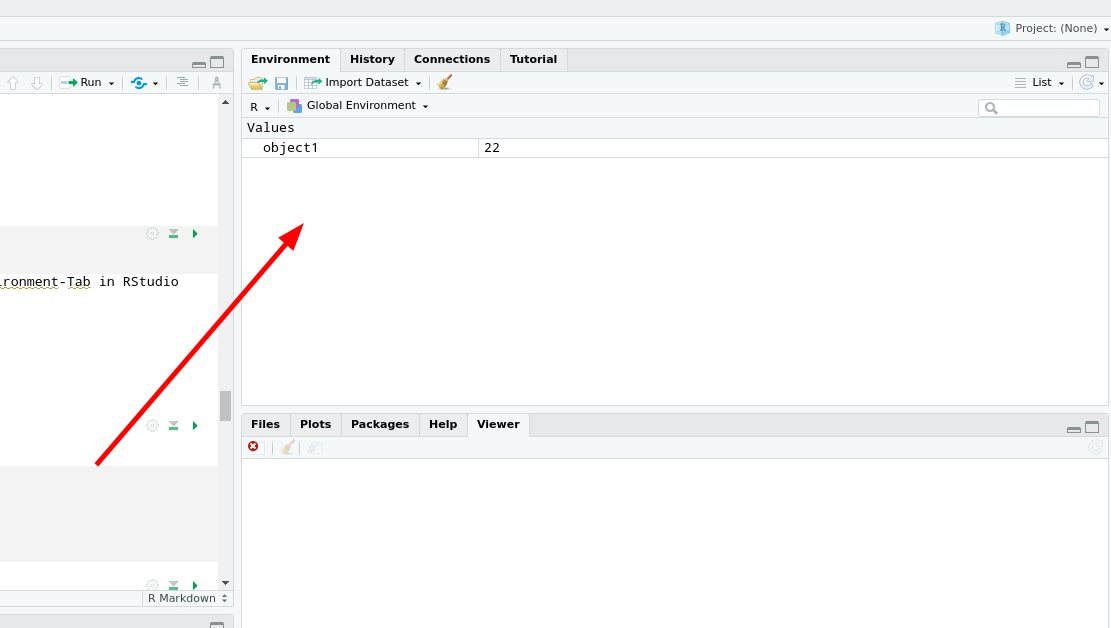
\includegraphics[width=0.4\textwidth,height=\textheight]{imgs/environment.png}
\caption{Environment}
\end{figure}

\hypertarget{objekte-entfernen}{%
\subsection*{Objekte entfernen}\label{objekte-entfernen}}
\addcontentsline{toc}{subsection}{Objekte entfernen}

Vorhandene Objekte lassen sich dann wie folgt entfernen:

\begin{Shaded}
\begin{Highlighting}[]
\KeywordTok{ls}\NormalTok{()}
\end{Highlighting}
\end{Shaded}

\begin{verbatim}
## [1] "a"           "firstObject" "object2"    
## [4] "plan"
\end{verbatim}

\begin{Shaded}
\begin{Highlighting}[]
\KeywordTok{rm}\NormalTok{(object2)}
\KeywordTok{ls}\NormalTok{()}
\end{Highlighting}
\end{Shaded}

\begin{verbatim}
## [1] "a"           "firstObject" "plan"
\end{verbatim}

Mit \texttt{rm(list=ls())} lassen sich alle Objekte aus dem Workspace entfernen.

\begin{Shaded}
\begin{Highlighting}[]
\KeywordTok{ls}\NormalTok{()}
\end{Highlighting}
\end{Shaded}

\begin{verbatim}
## [1] "a"           "firstObject" "plan"
\end{verbatim}

\begin{Shaded}
\begin{Highlighting}[]
\KeywordTok{rm}\NormalTok{(}\DataTypeTok{list=}\KeywordTok{ls}\NormalTok{())}
\KeywordTok{ls}\NormalTok{()}
\end{Highlighting}
\end{Shaded}

\begin{verbatim}
## character(0)
\end{verbatim}

\hypertarget{datentypen}{%
\subsection*{Datentypen}\label{datentypen}}
\addcontentsline{toc}{subsection}{Datentypen}

\small

In R, wie in so gut wie jeder anderen Sprache, werden Objekte in unterschiedliche Subtypen gegliedert, die sich auf die in ihnen gespeicherten Informationen beziehen:

\begin{tabular}[t]{l|l|l}
\hline
Beschreibung & Beispiel & Datentyp\\
\hline
leere Menge & `NULL` & `NULL`\\
\hline
logische Werte & `TRUE, FALSE, T,  F` & `logical`\\
\hline
ganze und reelle Zahlen & `42` & `numeric`\\
\hline
Buchstaben- o. Zeichenfolgen (immer in <br> Anführungszeichen) & `beware of the leopard.` & `character`\\
\hline
\end{tabular}

Dabei ist das hier keine vollständige Liste, für den Anfang reicht sie aber.

\texttt{mode()} gibt den Datentyp des übergebenen Arguments aus (braucht man selten, hier nur für das Beispiel):

\begin{Shaded}
\begin{Highlighting}[]
\KeywordTok{mode}\NormalTok{(answer)}
\end{Highlighting}
\end{Shaded}

\begin{verbatim}
## [1] "numeric"
\end{verbatim}

\begin{Shaded}
\begin{Highlighting}[]
\KeywordTok{mode}\NormalTok{(}\StringTok{\textquotesingle{}answer\textquotesingle{}}\NormalTok{)}
\end{Highlighting}
\end{Shaded}

\begin{verbatim}
## [1] "character"
\end{verbatim}

\hypertarget{datentypen-konvertieren}{%
\subsection*{Datentypen konvertieren}\label{datentypen-konvertieren}}
\addcontentsline{toc}{subsection}{Datentypen konvertieren}

\scriptsize

\texttt{as.character(answer)} konvertiert den Datentyp des Objekts von \texttt{numeric} nach \texttt{character} ohne den ursprünglichen Eintrag von \texttt{answer} zu überschreiben.

\begin{Shaded}
\begin{Highlighting}[]
\KeywordTok{mode}\NormalTok{(answer)}
\end{Highlighting}
\end{Shaded}

\begin{verbatim}
## [1] "numeric"
\end{verbatim}

\begin{Shaded}
\begin{Highlighting}[]
\KeywordTok{as.character}\NormalTok{(answer)}
\end{Highlighting}
\end{Shaded}

\begin{verbatim}
## [1] "42"
\end{verbatim}

\begin{Shaded}
\begin{Highlighting}[]
\KeywordTok{mode}\NormalTok{(answer)}
\end{Highlighting}
\end{Shaded}

\begin{verbatim}
## [1] "numeric"
\end{verbatim}

Um das zu erreichen muss das Objekt überschrieben werden:

\begin{Shaded}
\begin{Highlighting}[]
\NormalTok{answer \textless{}{-}}\StringTok{ }\KeywordTok{as.character}\NormalTok{(answer)}
\KeywordTok{mode}\NormalTok{(answer)}
\end{Highlighting}
\end{Shaded}

\begin{verbatim}
## [1] "character"
\end{verbatim}

Mit \texttt{answer} als character-Element lässt sich nicht mehr rechnen:

\begin{Shaded}
\begin{Highlighting}[]
\NormalTok{answer }\OperatorTok{*}\StringTok{ }\DecValTok{2}
\end{Highlighting}
\end{Shaded}

\begin{verbatim}
## Error in answer * 2: non-numeric argument to binary operator
\end{verbatim}

Um das dann wieder zu ermöglichen muss das Objekt zurück nach numeric konvertiert werden:

\begin{Shaded}
\begin{Highlighting}[]
\NormalTok{answer \textless{}{-}}\StringTok{ }\KeywordTok{as.numeric}\NormalTok{(answer)}
\KeywordTok{mode}\NormalTok{(answer)}
\end{Highlighting}
\end{Shaded}

\begin{verbatim}
## [1] "numeric"
\end{verbatim}

\begin{Shaded}
\begin{Highlighting}[]
\NormalTok{answer }\OperatorTok{*}\StringTok{ }\DecValTok{2}
\end{Highlighting}
\end{Shaded}

\begin{verbatim}
## [1] 84
\end{verbatim}

Weitere Beispiele für Konvertierung:

\begin{Shaded}
\begin{Highlighting}[]
\KeywordTok{as.numeric}\NormalTok{(}\StringTok{"42"}\NormalTok{) }\CommentTok{\#\#\# konvertiert character nach numeric}
\end{Highlighting}
\end{Shaded}

\begin{verbatim}
## [1] 42
\end{verbatim}

\begin{Shaded}
\begin{Highlighting}[]
\KeywordTok{as.numeric}\NormalTok{(}\OtherTok{TRUE}\NormalTok{) }\CommentTok{\#\#\# konvertiert logical nach numeric}
\end{Highlighting}
\end{Shaded}

\begin{verbatim}
## [1] 1
\end{verbatim}

\begin{Shaded}
\begin{Highlighting}[]
\KeywordTok{as.logical}\NormalTok{(}\DecValTok{0}\NormalTok{)  }\CommentTok{\#\#\# konvertiert numeric nach logical}
\end{Highlighting}
\end{Shaded}

\begin{verbatim}
## [1] FALSE
\end{verbatim}

\begin{Shaded}
\begin{Highlighting}[]
\KeywordTok{as.logical}\NormalTok{(}\DecValTok{1}\NormalTok{)  }\CommentTok{\#\#\# konvertiert numeric nach logical }
\end{Highlighting}
\end{Shaded}

\begin{verbatim}
## [1] TRUE
\end{verbatim}

\begin{Shaded}
\begin{Highlighting}[]
\KeywordTok{as.logical}\NormalTok{(}\DecValTok{23}\NormalTok{)  }\CommentTok{\#\#\# konvertiert numeric nach logical}
\end{Highlighting}
\end{Shaded}

\begin{verbatim}
## [1] TRUE
\end{verbatim}

\begin{Shaded}
\begin{Highlighting}[]
\KeywordTok{as.logical}\NormalTok{(}\StringTok{"true"}\NormalTok{)  }\CommentTok{\#\#\# konvertiert character nach logical}
\end{Highlighting}
\end{Shaded}

\begin{verbatim}
## [1] TRUE
\end{verbatim}

\hypertarget{logische-werte-operatoren-und-verknuxfcpfungen}{%
\subsection*{Logische Werte, Operatoren und Verknüpfungen}\label{logische-werte-operatoren-und-verknuxfcpfungen}}
\addcontentsline{toc}{subsection}{Logische Werte, Operatoren und Verknüpfungen}

Logische Vergleiche, Verknüpfungen und andere Operatoren:

\begin{table}[H]
\centering\begingroup\fontsize{15}{17}\selectfont

\begin{tabular}[t]{l|l}
\hline
Operator & Operation\\
\hline
`==` & ist gleich\\
\hline
`!=` & ist ungleich\\
\hline
> & ist größer\\
\hline
>= & ist größer gleich\\
\hline
< & ist kleiner\\
\hline
<= & ist kleiner gleich\\
\hline
`!` & logisches NICHT\\
\hline
\& & logisches UND\\
\hline
`|` & logisches ODER\\
\hline
`isTRUE()` & gibt an, ob übergebenes Argument TRUE ist\\
\hline
 & \\
\hline
\end{tabular}
\endgroup{}
\end{table}

Das Ergebnis eines logischen Vergleichs sind logische Werte:\\
WAHR: \texttt{TRUE\ =\ T\ =\ 1}\\
FALSCH: \texttt{FALSE\ =\ F\ =\ 0}

Beispiele:

\begin{Shaded}
\begin{Highlighting}[]
\DecValTok{1} \OperatorTok{==}\StringTok{ }\DecValTok{2}
\end{Highlighting}
\end{Shaded}

\begin{verbatim}
## [1] FALSE
\end{verbatim}

\begin{Shaded}
\begin{Highlighting}[]
\DecValTok{1} \OperatorTok{!=}\StringTok{ }\DecValTok{2}
\end{Highlighting}
\end{Shaded}

\begin{verbatim}
## [1] TRUE
\end{verbatim}

\begin{Shaded}
\begin{Highlighting}[]
\DecValTok{1} \OperatorTok{\textless{}}\StringTok{ }\DecValTok{2}
\end{Highlighting}
\end{Shaded}

\begin{verbatim}
## [1] TRUE
\end{verbatim}

\begin{Shaded}
\begin{Highlighting}[]
\DecValTok{1} \OperatorTok{\textgreater{}=}\StringTok{ }\DecValTok{2}
\end{Highlighting}
\end{Shaded}

\begin{verbatim}
## [1] FALSE
\end{verbatim}

\begin{Shaded}
\begin{Highlighting}[]
\DecValTok{1}\OperatorTok{\textgreater{}}\DecValTok{2} \OperatorTok{\&}\StringTok{ }\DecValTok{1}\OperatorTok{\textless{}=}\DecValTok{3}
\end{Highlighting}
\end{Shaded}

\begin{verbatim}
## [1] FALSE
\end{verbatim}

\begin{Shaded}
\begin{Highlighting}[]
\DecValTok{2}\OperatorTok{\textgreater{}}\DecValTok{1} \OperatorTok{|}\StringTok{ }\DecValTok{1}\OperatorTok{!=}\DecValTok{1}
\end{Highlighting}
\end{Shaded}

\begin{verbatim}
## [1] TRUE
\end{verbatim}

\begin{Shaded}
\begin{Highlighting}[]
\DecValTok{6}\OperatorTok{\textgreater{}}\DecValTok{5} \OperatorTok{\&}\StringTok{ }\OperatorTok{!}\NormalTok{(}\DecValTok{2}\OperatorTok{\textless{}=}\DecValTok{1}\NormalTok{)}
\end{Highlighting}
\end{Shaded}

\begin{verbatim}
## [1] TRUE
\end{verbatim}

\begin{Shaded}
\begin{Highlighting}[]
\KeywordTok{isTRUE}\NormalTok{(}\DecValTok{1} \OperatorTok{==}\StringTok{ }\DecValTok{1}\NormalTok{)}
\end{Highlighting}
\end{Shaded}

\begin{verbatim}
## [1] TRUE
\end{verbatim}

\begin{Shaded}
\begin{Highlighting}[]
\NormalTok{(}\DecValTok{1} \OperatorTok{==}\StringTok{ }\DecValTok{1}\NormalTok{)}
\end{Highlighting}
\end{Shaded}

\begin{verbatim}
## [1] TRUE
\end{verbatim}

\hypertarget{aufgabe-1}{%
\subsection*{Aufgabe}\label{aufgabe-1}}
\addcontentsline{toc}{subsection}{Aufgabe}

\hypertarget{was-kommt-raus-1}{%
\subsubsection*{Was kommt raus?}\label{was-kommt-raus-1}}
\addcontentsline{toc}{subsubsection}{Was kommt raus?}

\begin{Shaded}
\begin{Highlighting}[]
\NormalTok{(}\DecValTok{2} \OperatorTok{\textgreater{}}\StringTok{ }\DecValTok{1} \OperatorTok{\&}\StringTok{ }\DecValTok{1} \OperatorTok{\textless{}}\StringTok{ }\DecValTok{3}\NormalTok{) }\OperatorTok{|}\StringTok{ }\DecValTok{1} \OperatorTok{!=}\StringTok{ }\DecValTok{1}
\end{Highlighting}
\end{Shaded}

\begin{enumerate}
\def\labelenumi{\Alph{enumi})}
\tightlist
\item
  \texttt{TRUE}
\item
  \texttt{FALSE}
\item
  \texttt{NULL}
\end{enumerate}

\hypertarget{umgang-mit-dezimalzahlen}{%
\subsection*{Umgang mit Dezimalzahlen:}\label{umgang-mit-dezimalzahlen}}
\addcontentsline{toc}{subsection}{Umgang mit Dezimalzahlen:}

\hypertarget{was-kommt-hier-raus}{%
\subsubsection*{Was kommt hier raus?}\label{was-kommt-hier-raus}}
\addcontentsline{toc}{subsubsection}{Was kommt hier raus?}

\begin{Shaded}
\begin{Highlighting}[]
\FloatTok{0.1} \OperatorTok{+}\StringTok{ }\FloatTok{0.2} \OperatorTok{==}\StringTok{ }\FloatTok{0.3}
\end{Highlighting}
\end{Shaded}

\begin{enumerate}
\def\labelenumi{\Alph{enumi})}
\tightlist
\item
  \texttt{TRUE}
\item
  \texttt{FALSE}
\item
  \texttt{NULL}
\end{enumerate}

\begin{Shaded}
\begin{Highlighting}[]
\FloatTok{0.1} \OperatorTok{+}\StringTok{ }\FloatTok{0.2} \OperatorTok{==}\StringTok{ }\FloatTok{0.3}
\end{Highlighting}
\end{Shaded}

\begin{verbatim}
## [1] FALSE
\end{verbatim}

\textbf{0.1 + 0.2 != 0.3?}

`Falsches' Ergebnis ist Resultat von Repräsentation von Gleitkommazahlen im Speicher des Rechners.\\
Die Funktion \texttt{all.equal()} löst dieses Problem.

\begin{Shaded}
\begin{Highlighting}[]
\KeywordTok{all.equal}\NormalTok{(}\DataTypeTok{target=}\FloatTok{0.1+0.2}\NormalTok{, }\DataTypeTok{current=}\FloatTok{0.3}\NormalTok{)}
\end{Highlighting}
\end{Shaded}

\begin{verbatim}
## [1] TRUE
\end{verbatim}

Mit dem \texttt{tolerance}-Argument lässt sich der Bereich der akzeptabeln Unterschiede in Dezimalstellen angeben.

\begin{Shaded}
\begin{Highlighting}[]
\KeywordTok{all.equal}\NormalTok{(}\DataTypeTok{target =} \FloatTok{0.424242}\NormalTok{, }\DataTypeTok{current =} \FloatTok{0.424243}\NormalTok{,}
          \DataTypeTok{tolerance =} \FloatTok{1e{-}5}\NormalTok{)}
\end{Highlighting}
\end{Shaded}

\begin{verbatim}
## [1] TRUE
\end{verbatim}

\begin{Shaded}
\begin{Highlighting}[]
\KeywordTok{all.equal}\NormalTok{(}\DataTypeTok{target =} \FloatTok{0.424242}\NormalTok{, }\DataTypeTok{current =} \FloatTok{0.424243}\NormalTok{,}
          \DataTypeTok{tolerance =} \FloatTok{1e{-}6}\NormalTok{)}
\end{Highlighting}
\end{Shaded}

\begin{verbatim}
## [1] "Mean relative difference: 2.357145e-06"
\end{verbatim}

Hierbei fällt auf, dass bei Ungleichheit nicht \texttt{FALSE} sondern die Abweichung ausgegeben wird.

Um \texttt{all.equal} sinnvoll in logischen Operationen benutzen zu können wird \texttt{isTRUE} benötigt:

\begin{Shaded}
\begin{Highlighting}[]
\KeywordTok{isTRUE}\NormalTok{(}\KeywordTok{all.equal}\NormalTok{(}\DataTypeTok{target =} \FloatTok{0.424242}\NormalTok{,}
                 \DataTypeTok{current =} \FloatTok{0.424243}\NormalTok{,}
                 \DataTypeTok{tolerance =} \FloatTok{1e{-}6}\NormalTok{))}
\end{Highlighting}
\end{Shaded}

\begin{verbatim}
## [1] FALSE
\end{verbatim}

\hypertarget{hausaufgabe}{%
\section{Hausaufgabe}\label{hausaufgabe}}

\hypertarget{hausaufgabe-erstellen-eines-r-skripts}{%
\subsection*{Hausaufgabe: Erstellen eines R-Skripts}\label{hausaufgabe-erstellen-eines-r-skripts}}
\addcontentsline{toc}{subsection}{Hausaufgabe: Erstellen eines R-Skripts}

Schreiben Sie den dem folgenden Ablauf entsprechenden Code in ein R-\emph{Skript} und führen Sie ihn von dort in der Konsole aus:

Erstellen Sie drei Objekte wie folgt:

\begin{itemize}
\item
  Als erstes ein Objekt namens \emph{whatDoIDoThis} mit der Zahl 4 als Inhalt.
\item
  Als zweites ein Objekt namens \emph{text} mit dem Inhalt : ``i\_like\_snake\_case\_better''.
\item
  Als drittes ein Objekt namens \emph{myFavouriteNumber} mit einer Zahl Ihrer Wahl als Inhalt.
\end{itemize}

Berechnen Sie nun den Mittelwert der Objekte mit numerischem Inhalt und legen Sie diesen in einem weiteren Objekt namens \emph{manualMean} ab.

Lassen Sie sich in der Konsole durch eine Zeile in Ihrem Skript den Text \texttt{\textquotesingle{}I\ learned\ about\ the\ most\ important\ bugfixing\ tool\textquotesingle{}} ausgeben.

Speichern Sie anschließend das R-\emph{Skript} unter `.R' ab.

  \bibliography{book.bib,packages.bib}

\end{document}
